Most quantum processors are currently based on qubits.
Quantum computing based on $3$-level systems is known to offer many advantages over qubit-based quantum computing.
As an example, error correction can be done more efficiently \cite{campbell14} and quantum cryptography is more robust \cite{bechmann00}.
A qutrit processor has also recently been used to study thermalisation and loss of information in closed quantum systems \cite{blok20}.
In this chapter, I will introduce the reader to the basic concepts of $3$-level systems and discuss the challenge of generalizing the algorithm discussed in chapter 4 to qutrit systems.\\
First, we will look at the generalization of the Bloch representation to $d$-level systems.
We represent a state $\rho$ with the help of a $d^2-1$-dimensional Bloch vector $\bm{\tau}$.
We call the space of states that fulfill the conditions presented in chapter 1 the Bloch space.
A state $\rho$ can be represented in the following way:
$$\rho = \frac{1}{d} \1 + \sum_{i=1}^{d^2-1} \tau_i \sigma_i$$
where $\sigma_i$ are generators of $SU(d)$ obeying
\begin{equation}\label{sig}
	\sigma_i\sigma_j = \frac{2}{d}\delta_{ij} + d_{ijk}\sigma_k + if_{ijk}\sigma_k
\end{equation}
The $f_{ijk}$ and $d_{ijk}$ are the structure constants of the Lie-Algebra.
$f_{ijk}$ is totally antisymmetric and equals the Levi-Civita-Symbol for $d=2$, $d_{ijk}$ is totally symmetric and vanishing for $d=2$.
We can construct the generators as follows:\cite{kimura03}
 \[
\{\sigma_i\}^{d^2-1}_{i=1} = \{u_{jk},v_{jk},w_l\}
\]
where
$$
	u_{jk} = \ket{k}\bra{k}+\ket{k}\bra{j}, ~ v_{jk} = -i(\ket{j}\bra{k}-\ket{k}\bra{j}),
$$
$$
	w_l = \sqrt{\frac{2}{l(l+1}} \sum_{j=1}^{l} \left( \ket{j}\bra{j}-l\ket{l+1}\bra{l+1} \right),$$
	$$ 1\le j\le k\le d, 1\le l\le d-1.$$

\noindent The $\tau_i$ are the components of the Bloch vector and are the expectation values of the $\sigma_i$:
$$
	 \tau_i = Tr(\rho\sigma_i)
$$
The center of the Bloch space is the maximally mixed state $\rho_{*}=\frac{1}{d}\1$.
For $d\ge3$, there exist Bloch vectors with $\left|\tau\right|\le 1$ which do not correspond to a positive semi-definite matrix.
The space spanned by the Bloch-vectors is therefore not a solid ball with radius $1$.
We can deduce using \eqref{sig} the following conditions that we have to put on the Bloch vector for the density matrix to describe a pure state \cite{bengtsson17}:
\[
\rho=\rho^2\Leftrightarrow \begin{cases}
	\tau^2=\frac{d-1}{2d}\\
	d_{ijk}\tau_j\tau_k=\frac{d-2}{d}\tau_i
\end{cases}
.\]
The fist condition implies the Bloch vector of a pure state being confined to a $d^2-1$ dimensional outsphere.
The second condition says that the vectors of the pure states are a well defined subset of the surface of the outsphere.
The generators of  $SU(3)$ are the Gell-Mann-matrices $\lambda_i$: \[
\lambda_1=\begin{pmatrix} 0 & 1 & 0 \\ 1 & 0 & 0 \\ 0 & 0 & 0 \end{pmatrix},
\lambda_2=\begin{pmatrix} 0 & -i & 0 \\ i & 0 & 0 \\ 0 & 0 & 0 \end{pmatrix},
\lambda_3=\begin{pmatrix} 1 & 0 & 0 \\ 0 & -1 & 0 \\ 0 & 0 & 0 \end{pmatrix},
\] \[
\lambda_4=\begin{pmatrix} 0 & 0 & 1 \\ 0 & 0 & 0 \\ 1 & 0 & 0 \end{pmatrix},
\lambda_5=\begin{pmatrix} 0 & 0 & -i \\ 0 & 0 & 0 \\ i & 0 & 0 \end{pmatrix},
\lambda_6=\begin{pmatrix} 0 & 0 & 0 \\ 0 & 0 & 1 \\ 0 & 1 & 0 \end{pmatrix},\\
\]
\[
\lambda_7=\begin{pmatrix} 0 & 0 & 0 \\ 0 & 0 & -i \\ 0 & i & 0 \end{pmatrix},
\lambda_8=\frac{1}{\sqrt{3}} \begin{pmatrix} 1 & 0 & 0 \\ 0 & 1 & 0 \\ 0 & 0 & -2 \end{pmatrix}
.\]
They are traceless, hermitian, and obey $Tr\left(\lambda_i\lambda_j\right)=\delta_{ij}$.
The geometry of the Bloch space for qutrits has been studied by many authors \cite{mendas06,goyal16,kimura03} and many properties, such as sections in lower dimensions, have been found.
The problem with generalizing the algorithm shown by Bravyi \emph{et al.} to qutrits is that we can not directly map the solution states of the SDP to the Bloch space in the same way, since it is not a solid ball with radius one.
We therefore have to find a rounding scheme that takes into account the geometric restrictions of the Bloch space for three level systems.
An elgant and simple method to reduce the space to a solid ball in the Bloch space.
As proved in \cite{goyal16}, the boundary of the Bloch space of qutrits can never stray into the solid ball of radius $\frac{1}{2}$, meaning all bloch vectors with $ \left| \tau \right| \le \frac{1}{2}$ correspond to valid states.
This is proved by using that boundary vectors $\bm{\tau}\in\IR^{8}$ should necessarily satisfy \[
	det ~ \rho(\bm{\tau}) = 0
.\]
We can therefore apply the same rounding scheme as in the qubit case, modified for the smaller sphere.
The cut-off value therefore becomes $\frac{1}{2\sqrt{8}}$.
Visually, we fit a hypercube into the $8$-dimensional sphere of radius $\frac{1}{2}$ and round any states into the cube.
As a field study I have implemented this algorithm and plotted the result, mirroring the procedure described in chapter 4.
The model used is a one dimensional chain of the form: \[
H = \sum_{i=1}^{n}\lambda_1^{i}\lambda_1^{i+1}
\]
where $\lambda^{i}_{1}$ is the first Gell-Mann matrix operating on the $i$th qubit and the chain is closed, i.e. $\lambda^{n+1}_1=\lambda^{1}_1$.
The result can be seen in Figure \ref{fig:4}
\begin{figure}[H]
	\centering
	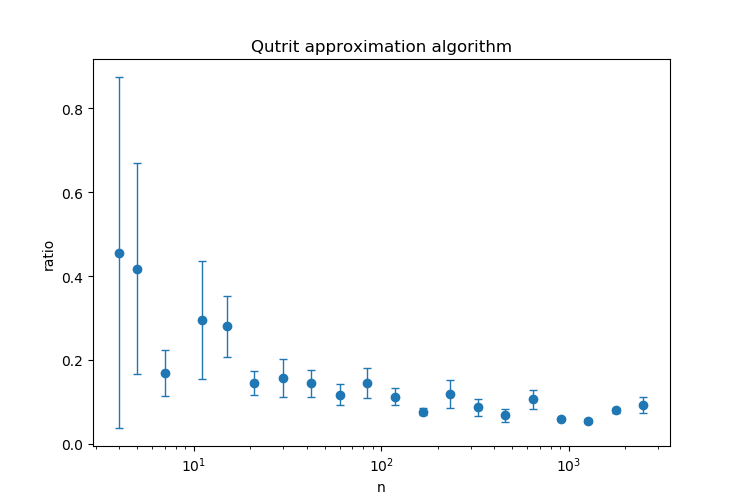
\includegraphics[width=0.8\textwidth]{tavgplot(4,2500,2,20,20).png}
	\caption{The result of the simplistically adapted algorithm on qutrits.}
	\label{fig:4}
\end{figure}
\noindent While the variance is very large for small $n$, it quickly falls off.
Next steps would include analytically proving the behaviour of the approximation ratio, and thinking about more efficient rounding schemes.
A better rounding scheme would include using the unique geometry of the Bloch space to make the cut-off smaller.
